%%%%%%%%%%%%%%%%%%%%%%%%%%%%%%%%%%%%%%%%%%%%%%%%%%%%%%%%%%%%%%%%%%%%
%% I, the copyright holder of this work, release this work into the
%% public domain. This applies worldwide. In some countries this may
%% not be legally possible; if so: I grant anyone the right to use
%% this work for any purpose, without any conditions, unless such
%% conditions are required by law.
%%%%%%%%%%%%%%%%%%%%%%%%%%%%%%%%%%%%%%%%%%%%%%%%%%%%%%%%%%%%%%%%%%%%

\documentclass[
  printed, %% The `digital` option enables the default options for the
           %% digital version of a document. Replace with `printed`
           %% to enable the default options for the printed version
           %% of a document.
  color,   %% Uncomment these lines (by removing the %% at the
           %% beginning) to use color in the digital version of your
           %% document
  notable, %% The `table` option causes the coloring of tables.
           %% Replace with `notable` to restore plain LaTeX tables.
  oneside, %% The `twoside` option enables double-sided typesetting.
           %% Use at least 120 g/m² paper to prevent show-through.
           %% Replace with `oneside` to use one-sided typesetting;
           %% use only if you don’t have access to a double-sided
           %% printer, or if one-sided typesetting is a formal
           %% requirement at your faculty.
  nolof,   %% The `lof` option prints the List of Figures. Replace
           %% with `nolof` to hide the List of Figures.
  nolot,   %% The `lot` option prints the List of Tables. Replace
           %% with `nolot` to hide the List of Tables.
  nocover,
  %% More options are listed in the user guide at
  %% <http://mirrors.ctan.org/macros/latex/contrib/fithesis/guide/mu/fi.pdf>.
]{fithesis3}
%% The following section sets up the locales used in the thesis.
\usepackage[resetfonts]{cmap} %% We need to load the T2A font encoding
\usepackage[T1,T2A]{fontenc}  %% to use the Cyrillic fonts with Russian texts.
\usepackage[
  main=english, %% By using `czech` or `slovak` as the main locale
                %% instead of `english`, you can typeset the thesis
                %% in either Czech or Slovak, respectively.
  english, czech %% The additional keys allow
]{babel}        %% foreign texts to be typeset as follows:
%%
%%   \begin{otherlanguage}{german}  ... \end{otherlanguage}
%%   \begin{otherlanguage}{russian} ... \end{otherlanguage}
%%   \begin{otherlanguage}{czech}   ... \end{otherlanguage}
%%   \begin{otherlanguage}{slovak}  ... \end{otherlanguage}
%%
%% For non-Latin scripts, it may be necessary to load additional
%% fonts:
\usepackage{paratype}
\def\textrussian#1{{\usefont{T2A}{PTSerif-TLF}{m}{rm}#1}}
%%
%% The following section sets up the metadata of the thesis.
\thesissetup{
    date        = \the\year/\the\month/\the\day,
    university  = mu,
    faculty     = fi,
    type        = bc,
    author      = Ondřej Svoboda,
    gender      = m,
    advisor     = {prof. RNDr. Jiří Barnat, Ph.D.},
    title       = {Simulating RoFI Platform in GazeboSim},
    TeXtitle    = {Simulating RoFI Platform in~GazeboSim},
    keywords    = {simulation, RoFI, GazeboSim, RoFI HAL, robots, modular, self-reconfigurable, docking, RoFICoM},
    TeXkeywords = {simulation, RoFI, GazeboSim, RoFI HAL, robots, modular, self-reconfigurable, docking, RoFICoM},
    abstract    = {%
A tool for simulating the distributed modular robotic platform RoFI is presented in this thesis.
The tool uses the Gazebo simulator as the base and extends its capabilities through the use of plugins.
This simulation is designed in such way, that it uses the same programming interface as the physical RoFI modules which allows to effortlessly transfer code between the physical modules and the simulation.
Moreover, the simulation keeps the distributed nature of the RoFI platform.
The thesis also includes a guide on how to run the simulation and it contains multiple examples.
    },
    thanks      = {%
        I would like to give my special thanks to Jan Mrázek as he provided the biggest support during the implementation of the work. I also want to thank my advisor Jiří Barnat for his patience and feedback. And last but not least, I would like to thank my sister who helped me with the formulation of my writing.
    },
    bib         = references.bib,
    assignment         = 
        blank.pdf,
        % assignment.pdf,
}
\usepackage{makeidx}      %% The `makeidx` package contains
\makeindex                %% helper commands for index typesetting.
%% These additional packages are used within the document:
\usepackage{paralist} %% Compact list environments
\usepackage{amsmath}  %% Mathematics
\usepackage{amsthm}
\usepackage{amsfonts}
\usepackage{url}      %% Hyperlinks
\usepackage{markdown} %% Lightweight markup
\usepackage{tabularx} %% Tables
\usepackage{tabu}
\usepackage{booktabs}
\usepackage{listings} %% Source code highlighting
\lstset{
  basicstyle      = \ttfamily,
  identifierstyle = \color{black},
  keywordstyle    = \color{blue},
  keywordstyle    = {[2]\color{cyan}},
  keywordstyle    = {[3]\color{olive}},
  stringstyle     = \color{teal},
  commentstyle    = \itshape\color{magenta},
  breaklines      = true,
}
\usepackage{floatrow} %% Putting captions above tables
\floatsetup[table]{capposition=top}

\newcommand{\code}[1]{\texttt{#1}}

\begin{document}
\chapter{Modular Robots}

Modular robots are robots that consist of different parts -- modules.
These modules can be connected in various ways to form a robot.
For example, a human-like robot can be modular by having different types of hands as modules.
There is not a clear distinction between what is a modular robot and what is just a robot that needs to be assembled. However, in general, if a robot can be assembled in multiple ways to perform different tasks, it can be called a modular robot.

Modular robots have the advantage of being able to perform various tasks depending on the modules used and the position in which the modules are connected.
Also, with multiple modules, if one of the modules break, there is no need to replace the whole robot, only the part that broke.
This enhances replaceability and significantly lowers the maintenance cost.

A major drawback is that robots that are specifically created for only one task can be more efficient in performing this task since they do not have to make any compromises.
This is why modular robots are not well suited for some specialized tasks such as work in manufactures and why they will probably never fully replace the regular ones.

\section{Self-reconfigurable robots}

Variations of modular robots are self-reconfigurable robots.
These are robots that can connect and disconnect without the help of an external force such as a human being unscrewing a module and screwing in a new one.
The idea of shapeshifting has been around for a long time and now it is possible within the robotics world with self-reconfigurable robots.
The robotic system's ability to change its shape according to the environment and task makes self-reconfigurable robots ideal for places where the circumstances are not known beforehand.

Self-reconfigurable robots consist of numerous modules that are connected together by a docking mechanism to form a combined robot.
Individual modules usually have on their own significantly reduced moving abilities, when connected together, they are capable of complex locomotions.
Self-reconfigurable robot platforms that focus on one or two main modules are called metamorphic.
With metamorphic robots, it is possible to have specialized modules, but, typically, the majority of a robot consists of the main modules.
Therefore, most of the reconfiguration of metamorphic robots is done by these main modules which can simplify the reconfiguration algorithms.

The origins of self-reconfigurable robots can be traced back to 1990 when CEBOT (Cellular Robotic System) started at Nagoya University in Japan.\cite{current-trends}
Since then, there have been many various designs of self-reconfigurable robots focusing on different aspects of possibilities that the robots have.
Some of these robotic designs include M-TRAN (up to M-TRAN III)\cite{mtran} that became an inspiration for a lot of other designs, SMORES\cite{smores} that enhances the mobility of a single module, and Roombots\cite{roombots} which features an original way to use robots in furniture.
However, throughout the years, there have been dozens and dozens of different designs of modular robots.\cite{current-trends}

For a combined robot to perform a complex task, the modules have to synchronize their movement.
This can be achieved by centralized or distributed control.
Centralized control selects a master module which then controls all of the other modules.
On the contrary, in distributed one, all modules control their own movement depending on the information from the entire combined robot.
The robot system can also use a combination of both controls, such as hierarchical control where the modules are divided into layers and each layer gives more precise commands to the layer beneath it.


\chapter{The RoFI Platform}
% Description of the RoFI platform, what is it made of, capabilities
% what it can do, what it can't do

\begin{figure}
    \centering
    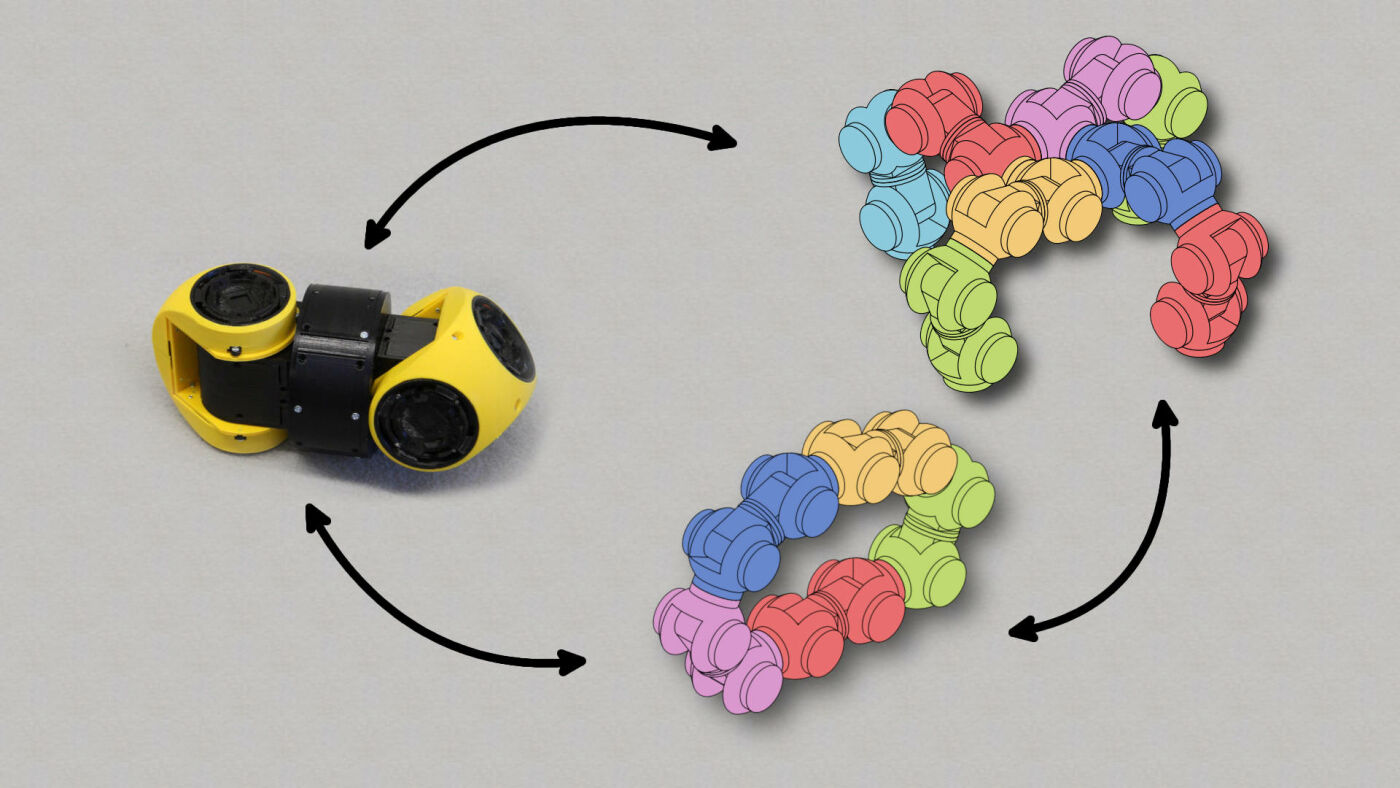
\includegraphics[width=\linewidth]{data/rofi_transformation.jpg}
    \caption{Image showing the reconfiguration capabilities of the RoFI platform. On the left side is a RoFI Universal Module. On the right side are two RoFIbots created by combining the RoFI Universal Modules. The figure has been taken from the RoFI website\cite{rofi-web}.}
    \label{fig:rofi-transform}
\end{figure}

RoFI is a platform for self-reconfigurable modular robots.
It is developed by a team in laboratory ParaDiSe\cite{paradise-web} at the Faculty of Informatics at Masaryk University.
All information about the RoFI project and things related to it are available at the projects website.\cite{rofi-web}
The RoFI platform was firstly presented in \emph{RoFI -- Distributed Metamorphic Robots}\cite{rofi-thesis} and had been evolving since then.

The platform specifies RoFI modules and RoFI connection mechanisms (RoFICoM).
RoFI modules connect together by RoFICoMs to create a combined robot which is referred to as a RoFIbot\label{rofibot} (see Figure \ref{fig:rofi-transform}).

\begin{figure}
    \centering
    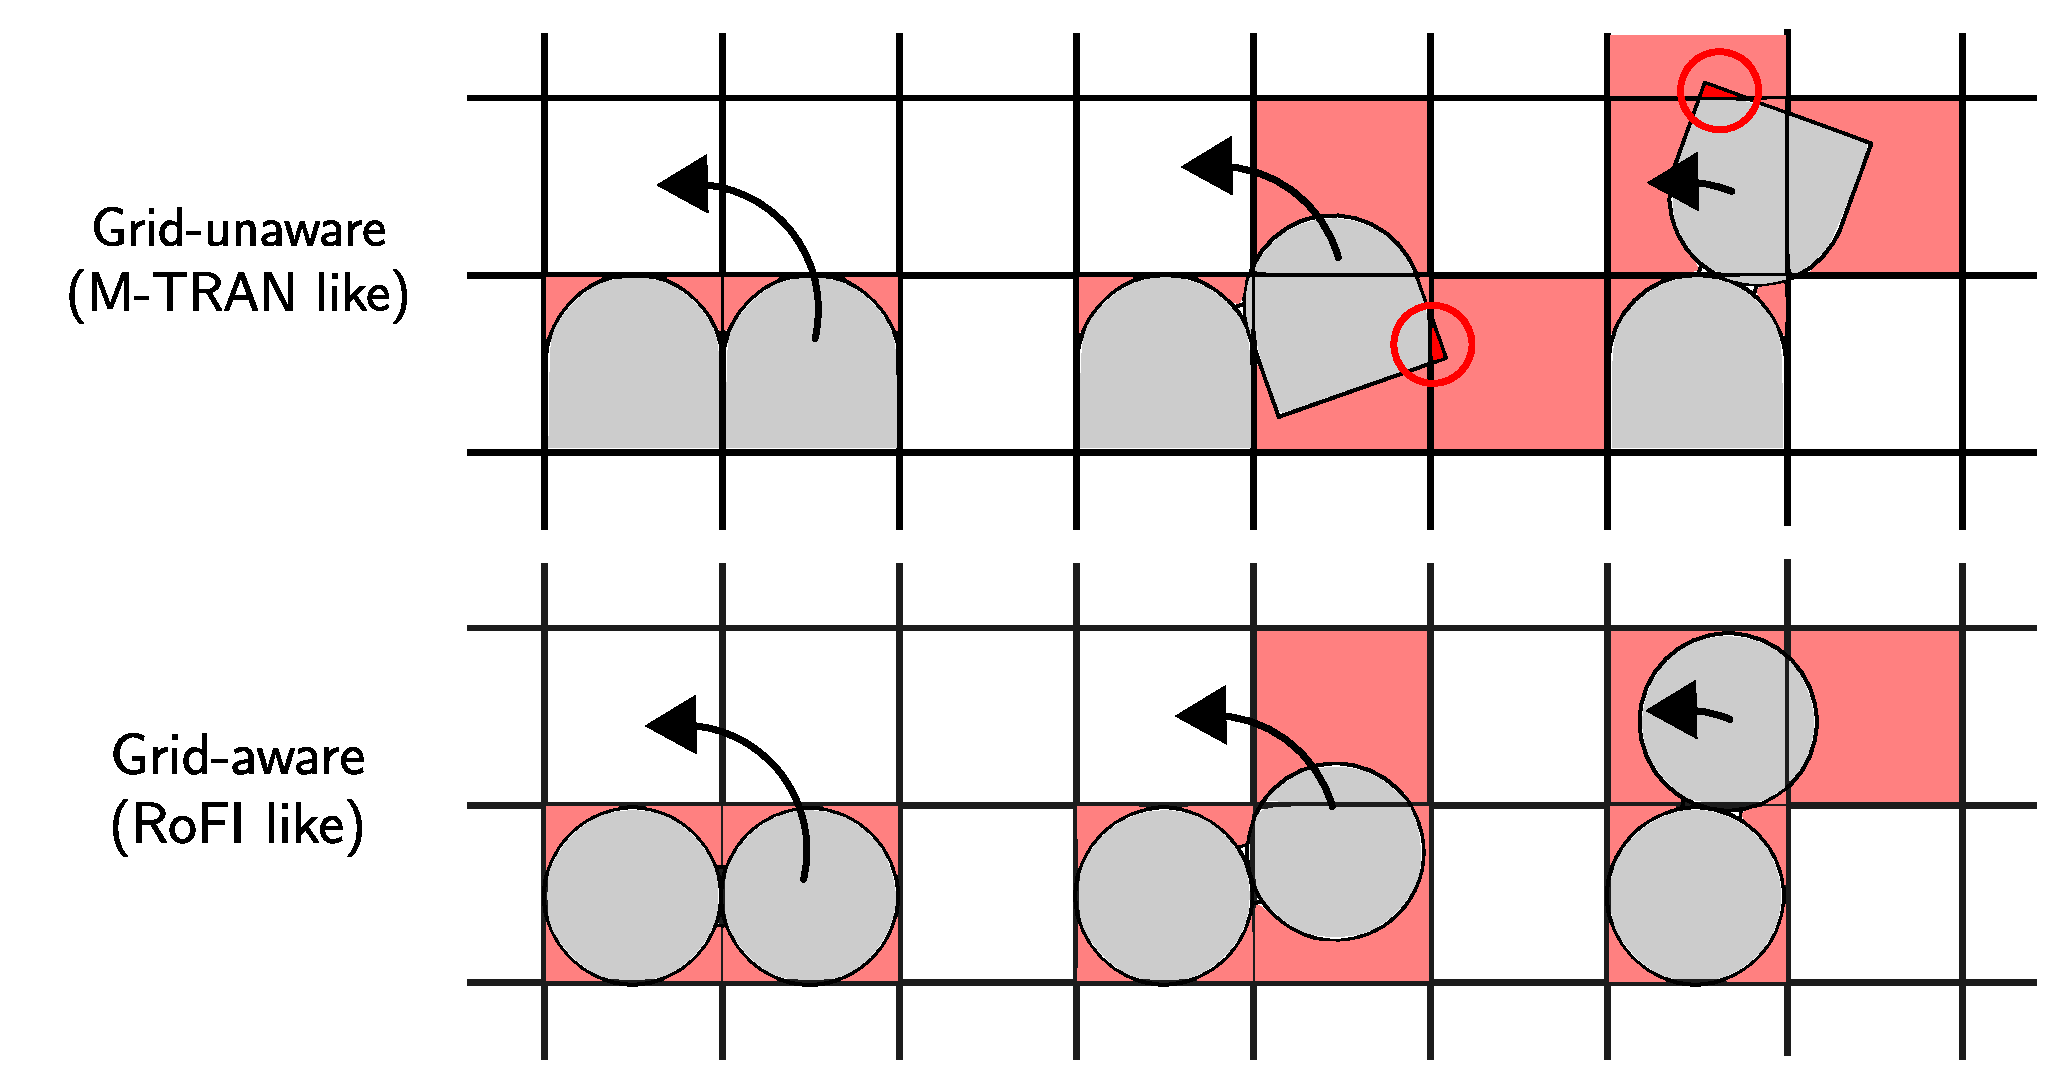
\includegraphics[width=\linewidth]{data/grid_aware.pdf}
    \caption{Comparison of grid-awareness in M-TRAN like and RoFI like systems. Figure taken from RoFI website\cite{rofi-web}.}
    \label{fig:grid-aware}
\end{figure}

The RoFI modules fit into a $10 \times 10 \times 10$ cm grid.
In order to allow RoFI modules to turn and change positions inside dense configurations, the RoFI modules are set to be grid-aware.
This removes additional constraints on the movement of modules and can simplify the algorithms for RoFI systems.
An example of such constraint is shown in Figure \ref{fig:grid-aware} which shows a rotation in RoFI compared to one in M-TRAN\cite{mtran} (a grid-unaware system).
In the example, the M-TRAN modules pass through more grid cells than necessary.
The RoFI provides the grid-awareness by allowing the modules to fill only a sphere inside each grid cell, and if a single module occupies two or more cells, it can also fill the space between them.

Each of the RoFI modules has its own control unit.
The control units of adjacent modules can communicate together through connected RoFICoMs by a predefined interface.
The RoFI platform has the opportunity of using distributed control because it allows for more effective utilization of the computational potential.
The RoFI also simplifies centralized control to a great extend with RoFI OS by providing a remote interface (see RoFI architecture diagram in Figure \ref{fig:architecture}).

The RoFI Hardware Abstraction Layer (HAL)\label{hal} allows users programming the RoFI module's code not to worry about the hardware's implementation details.
It provides control of the joints and connectors of a RoFI module and enables the users to register callbacks on events related to the module control.
Providing the same HAL interface in the simulator as well as in the physical RoFI modules permits using the same code for the physical modules and for the simulator and it allows to choose the target platform only by compiling the code with a different library.

\begin{figure}
    \centering
    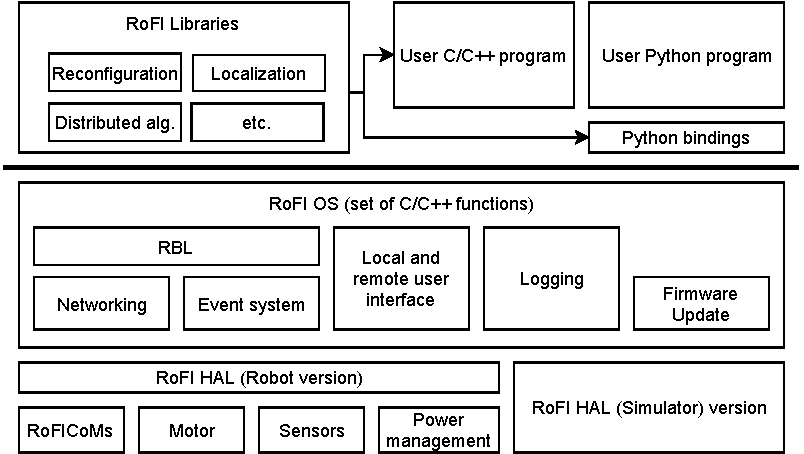
\includegraphics[width=\linewidth]{data/rofi_architecture.pdf}
    \caption{RoFI software architecture diagram. Diagram taken from RoFI website\cite{rofi-web}.}
    \label{fig:architecture}
\end{figure}

The RoFI robots are metamorphic which means that most of the modules are meant to be the same.
Nevertheless, having only one module notably limits the capabilities of the platform, so the RoFI platform allows for specialized RoFI modules.
These could have both an actuator and a sensor as long as they have the specified interface.
In order to handle all RoFI module shapes and capabilities, the RoFI platform defines module descriptors\cite{rofi-thesis}.
These descriptors provide abstractions of modules in graphs.
The abstractions enable to port existing algorithms onto the RoFI platform.

\section{RoFICoM}
\label{roficom}

\begin{figure}
    \centering
    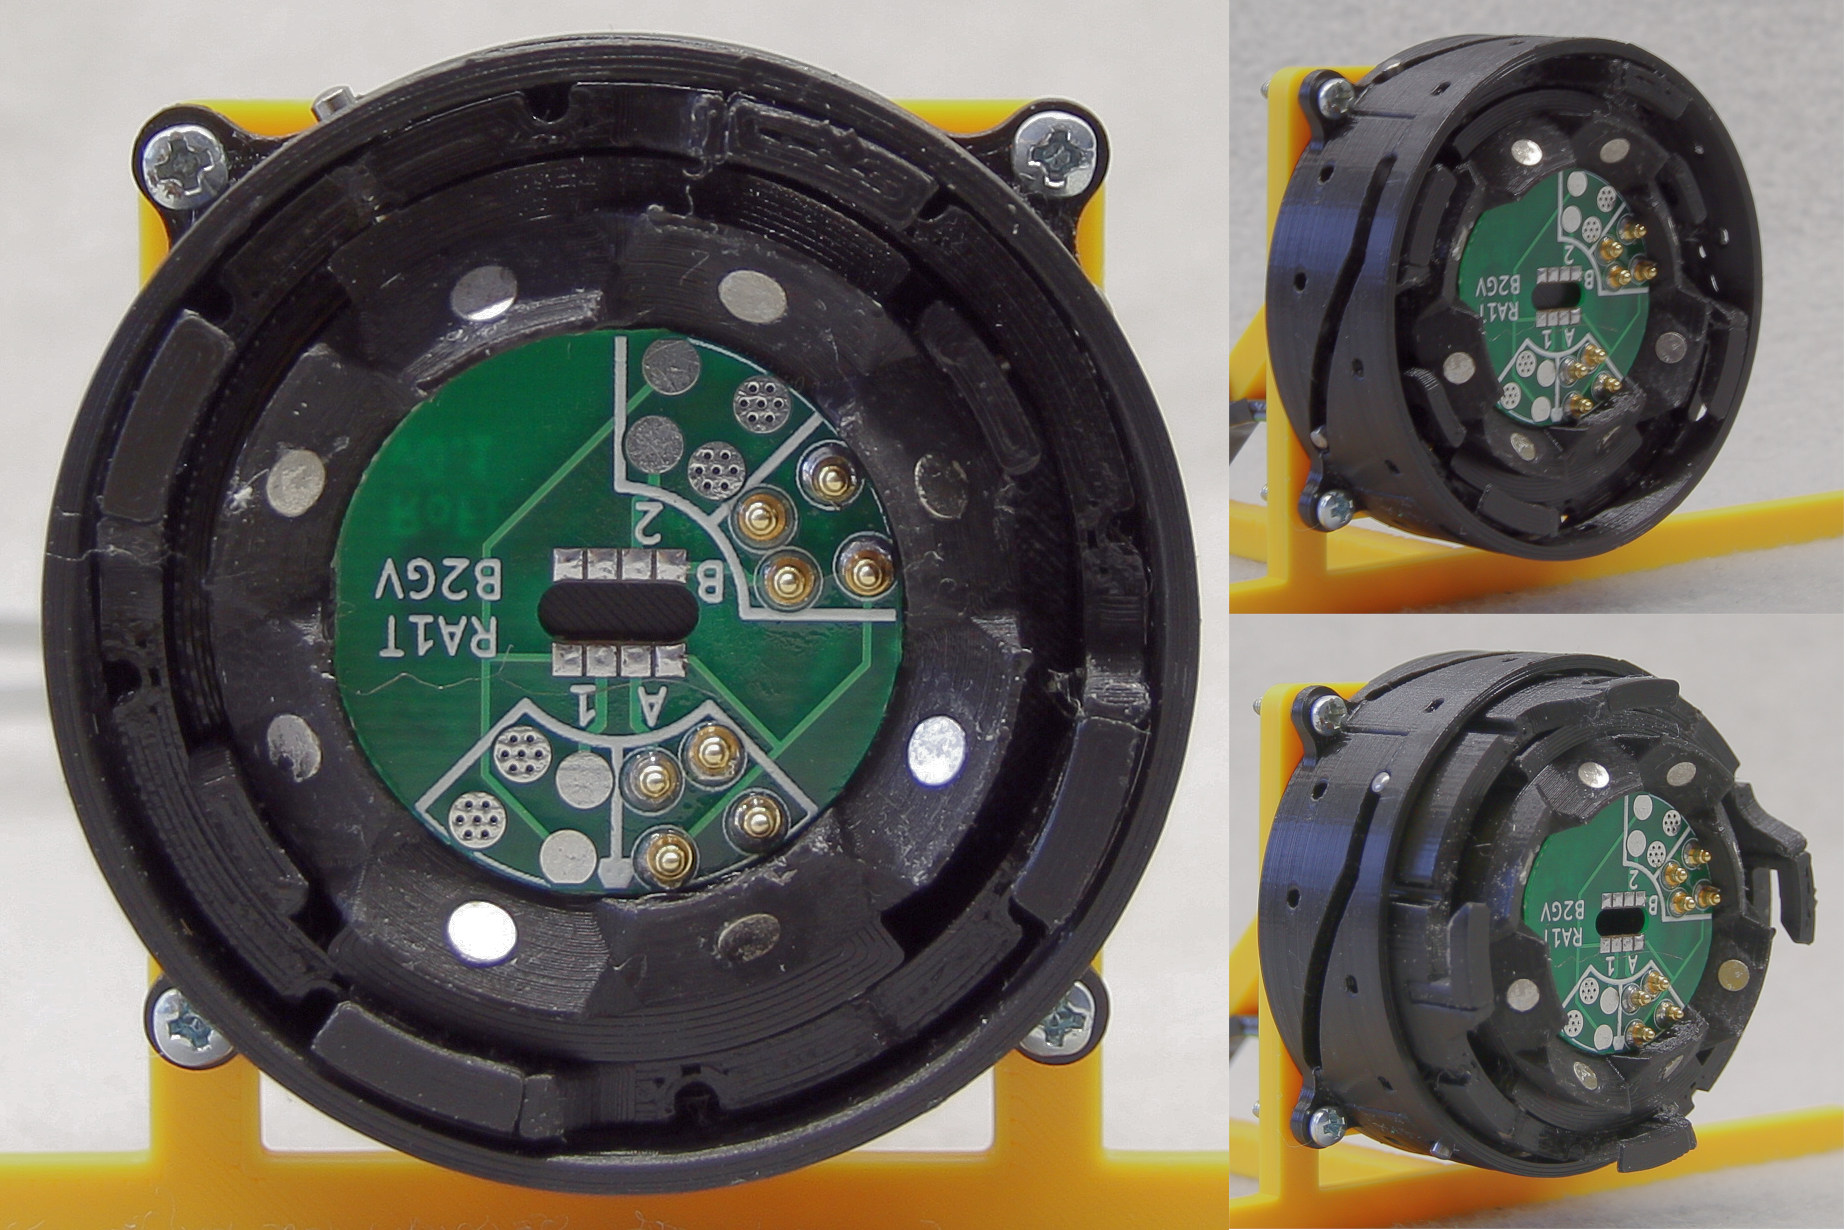
\includegraphics[width=\linewidth]{data/connector.jpg}
    \caption{RoFICoM from the front (left) and the difference between the RoFICoM in a retracted (right top) and extended (right bottom) state. Photo taken from RoFI website\cite{rofi-web}.}
    \label{fig:connector}
\end{figure}

Since the RoFI platform is designed to be grid-aware, the docking mechanisms of most of the other self-reconfigurable robots, such as M-TRAN\cite{mtran} or SMORES\cite{smores}, cannot be used.
In order to the connection being inside the grid cell sphere and having a stable connection surface, the connector has to be retractable.
The RoFI connection mechanism (RoFICoM) is a retractable docking mechanism that allows creating a stable connection between two RoFI modules.

In order to increase the flexibility of the RoFI system, the RoFICoMs are created genderless which means that any two RoFICoMs can be connected together.
The RoFICoM respects that the grid is cubical, and therefore, can be connected in four different orientations.
These orientations are north, east, west, and south and are the same from the perspectives of both connected RoFICoMs.

Since the connection between two modules is frequent and essential for the modular system, it is required not to drain energy in the connected state.
This eliminates the use of docks based on electromagnets.
The RoFICoMs are taking advantage of the need to be retractable with using a hooking system to create the connection.
This connection does not drain any energy except for when the RoFICoM is either extending or retracting.
The hooking system means that a RoFICoM can connect to another one nearby when either both RoFICoMs are extending, or one RoFICoM is extending and the other one is already extended.
To deal with potential dead modules, the RoFICoM connection can be disconnected by any of the two mating sides without the assistance of the other module.
The unnecessity of any action from the opposite side makes it possible to create a floor of extended RoFICoM-like hooks, to which the modules can connect.

The mechanical construction of RoFICoMs nullifies the possibility of connecting in a wrong angle -- either the RoFICoMs connect and align perfectly in one orientation or do not connect at all.
The construction allows some tolerance on the positioning and alignments of the connecting RoFICoMs.
The area of acceptance for RoFICoMs is discussed in "RoFICoM -- First Open-Hardware Connector for Metamorphic Robots"\cite[p. 6]{roficom}.

RoFICoM has several pins in the middle of the connecting plane.
These pins enable communication between RoFICoMs, sensing the connected RoFICoMs, and power-sharing.
The communication protocol between RoFICoMs allows sending data with error detection.
The sensing pin lets the RoFICoM to check if any RoFICoM is connected to it and if so, the pin can also detect the orientation of the connection.
The power-sharing property allows the RoFI module to charge other modules or to be charged by them.
It also allows it to enter into a survivor mode where it is powered by other modules and is only used to pass on packets.
More information about the capabilities of a RoFICoM can be found in "RoFICoM -- First Open-Hardware Connector for Metamorphic Robots"\cite{roficom} and on the RoFI website\cite{rofi-web}.

\section{Universal Module}
\label{univ-module}

\begin{figure}
    \centering
    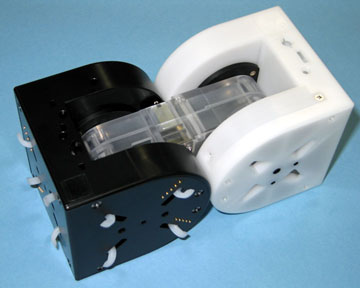
\includegraphics[height=.3\textheight]{data/mtran3.jpg}
    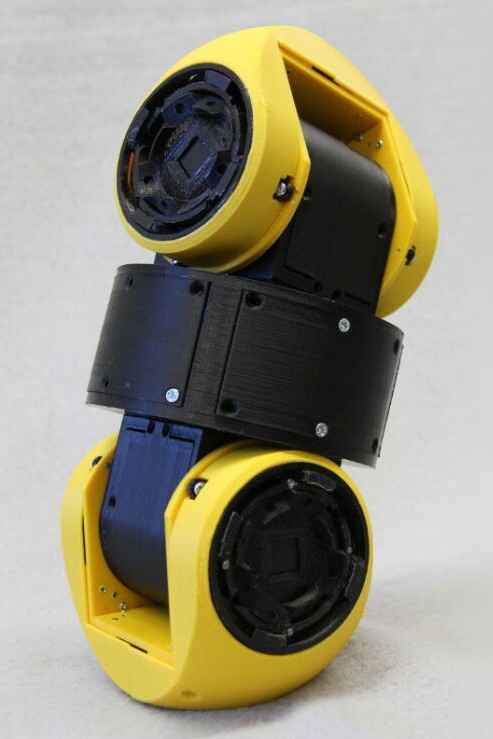
\includegraphics[height=.4\textheight]{data/rofi_universal_module.jpg}
    \caption{Comparison of an M-TRAN module (left) with a RoFI Universal Module (right). Photos taken from M-TRAN website\cite{mtran-web} and RoFI website\cite{rofi-web}.}
    \label{fig:mtran-rofi}
\end{figure}

\begin{figure}
    \centering
    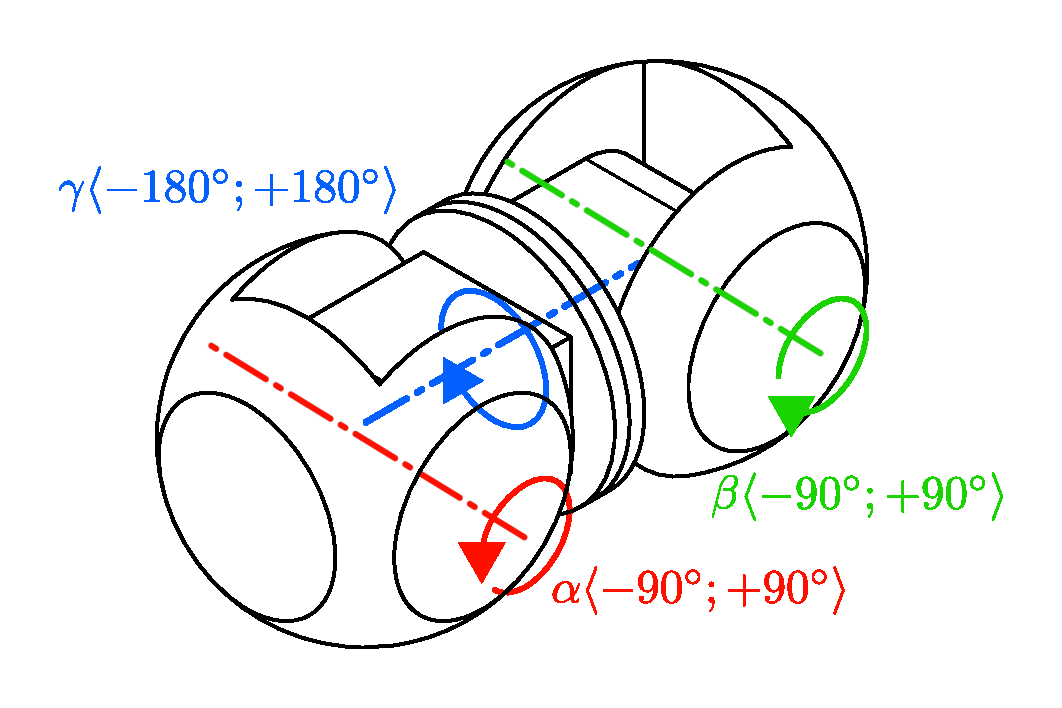
\includegraphics[height=.4\textheight]{data/rofi_universal_module_dof.pdf}
    \caption{Illustration of three degrees of freedom in the RoFI Universal Module. Picture taken from RoFI website\cite{rofi-web}.}
    \label{fig:univ-module-dof}
\end{figure}

The Universal Module is a RoFI module which serves as the primary building block of the RoFI platform.
The Universal Module is inspired by the M-TRAN\cite{mtran} module.
The comparison of the two modules can be seen in Figure \ref{fig:mtran-rofi}.
The M-TRAN and RoFI modules are composed of two shoes that each occupy one grid cell and are connected together by the body.
Each shoe can rotate around its axis.
The RoFI Universal Module has, in comparison to M-TRAN, an additional rotational axis going through the middle of the module body (see Figure \ref{fig:univ-module-dof}).
The range of motion allows each shoe to have three connectors.
Note, that M-TRAN has gendered connectors, whereas RoFI has them genderless.

The RoFI Universal Module uses ESP32 microprocessor as the control unit.
The ESP32 provides a POSIX-compatible interface and the full C++ standard library, simplifying the software development for Universal Modules.
The module utilizes servo-motors for rotation.
The servo-motors allow the controlling of the module's joints by position and speed on top of the force.
This allows the distribution of the control unit's responsibilities and speeds up the development of the RoFI platform.


\chapter{Robotics Simulator}
% What is a robotics simulator (for those, who never heard of it)
% Why is it beneficial, what are advantages/disadvantages

A robotics simulator is a computer software that enables the programmer or designer to observe how a robot behaves in different environments.
Naturally, using a virtual robot nullifies any possibility of breaking the physical robot and allows testing the robots in diverse environments and robot quantities -- which would be costly, especially in the beginning of a robot's development.
The simulator also lets the programmer test the robot without the necessity of having a physical robot at hand.

Simulators provide various tools that enable and simplify the robotic simulations.
The most crucial ability is to calculate the physics of the simulated world which is done by the physics engine.
Besides computing physics, the simulator provides a way to display the simulation graphically.
Most of the simulators also have an easy way to interact with the simulation.
If we assume that the simulation has multiple models which include the robots and a set environment (floor, obstacles, \ldots), then the interactions include moving, rotating, and scaling the models, adding new models, or changing some properties of the simulated models (such as, if the model is affected by gravity).

% physics engine
The simulator uses a physics engine to compute the underlying physics interactions.
There are two main ideas behind the physics engine -- a real-time and a high-precision physics engine.
This division is made by the fact that a simulation is never 100\% accurate, due to the rounding up of floating-point numbers and the imperfections of the physics model.
The real-time simulation is often used in video games (which use physics of some kind), and also in general, when the user interaction and response time is more important than the precision of the simulation.
The high-precision, on the other hand, is used a lot in scientific simulations.
These physics engines use a higher number of iterations and more precise calculations to provide more accurate simulations at the possible expense of the simulations going slower.

The simulators commonly include a way how to add a new model template.
This enables the user to specify the properties of the model in one place.
Since the simulation gets more difficult to compute when using more complex shapes, the simulators offer the possibility to add a different collision body than the visual.
Using a simplified collision body enables the simulation to run more smoothly while looking the same.

The Gazebo simulator\cite{gazebo} is one of the most widely used open-source robotics simulators.
Here, it will be used to demonstrate a way of defining objects in a simulation.
The GazeboSim utilizes a Simulation Description Format (SDFormat)\cite{sdf}.
A world in SDFormat contains models (objects in the simulation), plugins (third party extension software), and settings like gravity, wind, light, physics engine, and GUI.
The SDFormat world can also include a state which holds information about the models' times and current positions.
Each model in SDFormat consists of any number of links, joints, plugins, and even other models.
The links are the objects in the simulation that have weight and body.
The joints can connect two links and create a constraint on the links' relative movement to each other.
The joints are of multiple types, including a fixed joint, a prismatic joint (the links there can slide in one direction), and a revolute joint (the links there can rotate around an axis).

When designing a new robot, the process can be split into few steps:
\begin{enumerate}
    \item Specify the requirements for the robot.
    \item Create a robot design based on the requirements.
    \item Create the robot.\label{item:create-robot}
    It can be created physically or possibly in a simulator.
    \item Test the robot in various environments to see if it fulfills the needs.\label{item:test-robot}
    \item If the needs are not met, tweak the design based on the observations from the testing and go back to step \ref{item:create-robot}.
\end{enumerate}
Without using a simulator, the steps \ref{item:create-robot} and \ref{item:test-robot} would be costly and perhaps not even possible.
When using a simulator, especially in the early stage of the development, the step \ref{item:create-robot} becomes much cheaper and possibly less time-consuming and the step \ref{item:test-robot} becomes much more manageable to execute.

In the case of writing a new program for a robot, the steps remain similar to the designing of a robot.
The main difference is that there are no additional costs associated with creating a new program, but on the contrary, the simulator helps significantly more in the testing step.

\section{Simulators for Self-Reconfigurable Robots}
% What is the difference against normal simulator

Self-reconfigurable robot systems usually have multiple modules and even the interaction between the modules can have a significant impact on the behavior of the system on the outside.
Testing programs for these robots is, therefore, even more crucial, since the outcome of a user's code is not clear.
This makes having a simulator more valuable, but there are also obstacles in creating such a simulator which would not arise while simulating regular robots.

Self-reconfigurable robots depend heavily on the connection between the modules and it has often very complicated mechanisms to ensure stability.
If the connection system was created as the one in the real world, these mechanisms would often cause a computational overload for the simulator and the imperfection of the physics model would probably cause instabilities in the simulation.
However, for the aim of the simulation, the simulator can ignore these mechanisms and only reflect the outcomes of the connections.

% What robotics simulators exist
% Why do we need a new thing
One example of a simulator for self-reconfigurable robots is the Unified Simulator for Self-Reconfigurable Robots\cite{ussr} which addresses the connectivity problem and supports a great number of modules in a simulation.
These simulators often try to solve more aspects of the simulating of self-reconfigurable robots at the same time but at the cost of precision and user-friendliness.
Most of these simulators have not received an update for years, so lack of evolution and support is a substantial drawback for them.

\section{Simulator selection}
% available simulators

There are few options for choosing a simulator and addressing the constraints related to the simulating of modular robots:
\begin{enumerate}
    \item Use a dedicated simulator for self-reconfigurable robots.
    This could be either one already created or it could be made from scratch.
    \item Use a generic simulator and add to it the required capabilities.
\end{enumerate}

SMORES\cite{smores} team in their presentation of the platform\cite{smores-video} use for simulating Unity, however, the SMORES modules are not reconfiguring in the presentation.
Thereby, it seems that they did not address the reconfiguration issue at all.

The main reasons to use a generic robotics simulator are the continuous improvement of the simulator, the developers support, and the large community.
A lot of teams design robots in these days.
Most of them use a simulator of some kind, so it is reasonable to assume that robotics simulators largely used today will continue to progress and be supported in the future.
These simulators have a way to customize or extend the functionality of themselves by using plugins such as GazeboSim\cite{gazebo} and Webots\cite{webots}, or macros such as RoboDK\cite{robodk}.

This thesis is using the Gazebo simulator (GazeboSim).
The reasons for choosing GazeboSim as the platform are:
\begin{itemize}
    \item \emph{The community support.}\\
    The Gazebo simulator is used for the Robotic Operating System\cite{ros}, which is a growing platform for helping with robot development.
    This indicates that the simulator will stay supported for a significant time and will probably be further developed.
    \item \emph{The variety of supported physics engines.}\\
    GazeboSim allows the user to choose between multiple physics engines that offer variable precision and time complexity when computing the simulation.
    \item \emph{The server-client based simulation.}\\
    GazeboSim is based on the server-client model where all the difficult and resources-heavy computations are performed on the server-side and the visuals are presented on the client-side.
    This separation enables to run the simulation on a remote computer or to run it in a headless (server only) mode which could be used, e.g., for training AI.
    For the communication between the server and client, GazeboSim uses Protocol Buffers (Protobuf) messages\cite{protobuf} that provide a concise representation of data.
    \item \emph{The C++ API.}\\
    The RoFI platform software is developed in C++, so it is convenient to have the simulator API in the same programming language.
    \item \emph{The software license.}\\
    GazeboSim is developed under the open-source Apache 2.0 license which suits well with the intention of the RoFI team to have the work available to everyone.
\end{itemize}

There are a couple of challenges that arose during the work with GazeboSim and are not common when simulating regular robots:
\begin{itemize}
    \item \emph{Simulating the user code in the RoFI modules.}
    \item \emph{Connecting RoFICoMs in the simulation.}
    \item \emph{Distributing the RoFI modules.}
    \item \emph{Controlling RoFI joints by position and velocity.}
    \item \emph{Publishing control messages from multiple threads.}
    \item \emph{Saving and loading worlds.}
    \item \emph{Handling simulation wall-clock time.}
\end{itemize}
% TODO rozvest


\chapter{RoFI Simulator Design}

\section{Overall Design}
% why client/server
% other posibility: compilating to plugin
% why one process/one rofi (e.g. SIGKILL)
% why HAL
% diagram about interfaces - where stands gazebo, plugins, models, user code, hal, ...

% pid controller
% messages

% TODO diagram of simulator design

The aim of the design is to create a simulator for the RoFI platform.
The design should be able to execute the same user's code in the physical RoFI modules and in the simulation.
This would allow an easy development and debugging of the code for the real modules, without the possibility of breaking them.
The simulator should also keep the distributed nature of the RoFI modules.

\subsection{HAL Interface}

As shown in Figure \ref{fig:architecture}, the RoFI platform uses HAL (see Section \ref{hal}) to interact with the physical RoFI module.
The ability to use the same user's code in both, the physical RoFI and in the simulated one, can be achieved by providing the HAL interface to the simulation.
The compiling of the code can then be done by creating two targets and linking them with the appropriate libraries.
Since the HAL is directly above the hardware of the physical module, the simulator can also be used to test the RoFI OS and the RoFI libraries (as shown in Figure \ref{fig:architecture}).

\subsection{RoFICoM Model}

The RoFICoM (see Section \ref{roficom}) is a crucial component to all RoFI modules and in most of the modules it is featured multiple times.
Because of this and because RoFICoM has many unique properties, it is convenient to have an isolated RoFICoM model.
This also allows distributing the work from the RoFI module plugin to several RoFICoM plugins.

The communication between the RoFI module plugin and RoFICoM plugins is done by Protobuf messages.
Gazebo allows only for unique scoped names of models, so the communication topics are chosen to be the scoped names of the RoFICoM models, because both plugins have access to the RoFICoM model.

It is expected that only the RoFICoM model is going to have the RoFICoM plugin attached.
However, for the purpose of a simulation, any Gazebo model which has the RoFICoM plugin attached to it is considered to be a RoFICoM.

\subsection{Creating Modules}

The only module that the RoFI platform specifies at the time of writing this thesis is the Universal Module (see Section \ref{univ-module}).
Nevertheless, since the RoFI platform allows any number of different RoFI modules, there is an easy way to create a new module (see an example in Section \ref{ex-modules}).

Any Gazebo model with the RoFI module plugin attached to it is considered to be a RoFI module.
This is consistent with the RoFICoM, although it is expected that the simulation can have multiple different RoFI modules.

The simulation assumes all SDFormat children of a RoFI module which have a RoFICoM plugin to be RoFICoMs of the given module (in the order in which they appear in the SDFormat).
The joints that the RoFI module controls have to be specified in the RoFI module plugin.
This allows for joints that are not controlled by the RoFI module, if such need arises.

\section{Challenges}
% difficulties in the design: what needs to be done, clients, connecting roficoms, saving world and reloading (saving plugin info to sdf), waiting

During the implementation, there were a few challenges to overcome.
Here are some of the more important ones with an outline of the solutions and reasoning behind them.

\subsection{Simulating the User Code in the RoFI Modules}

Gazebo allows extending its functionality by various plugins.
The usual approach using GazeboSim is to have each robot have its own SDFormat model and to control it using a model plugin attached to it.
This plugin can directly control the robot or it can serve as a middle-man for an external program.

One possible way to simulate the user code in the RoFI module is to compile each RoFI program into a separate model plugin.
Then at the start of the simulation, the corresponding plugin has to be attached to each RoFI module.
This approach makes the implementation reasonably simple since it mostly just copies the physical implementation.
However, there are some flaws in this design as well:
\begin{itemize}
    \item When the user program fails and terminates (e.g., because of a SIGKILL), the whole simulation would collapse because Gazebo runs all plugins in the same process.
    \item In case of different codes, each generated plugin would have to be available to Gazebo and specified with its unique name in the world description.
    This would get tedious as the number of modules increases.
    \item It eliminates (or makes especially difficult) the possibility of changing the code during the simulation.
    \item There would be no simple way to include a new RoFI module in the simulation while running because there would be no default plugin to attach and it also cannot be changed later.
\end{itemize}

The other design used in this thesis is making use of the plugin as the middle-man for a separate program.
The model plugin interprets the Protobuf command messages and controls the RoFI module in the Gazebo simulation.
The user program is a thin layer that translates the RoFI HAL commands to the Protobuf command messages which can then be processed by the plugin.
This design allows to separate the processes of each module and thus to keep the distributed nature of the RoFI modules.
The separation of processes could also be used to imitate the limited capabilities of the microprocessor used in RoFI modules.
Nevertheless, there are some negative elements that have to be considered in this approach:
\begin{itemize}
    \item There is no guarantee that a message will arrive.
    \item Even if the messages arrive, they could be delayed or reordered.
    \item Both the program and plugin have to share a common topic name which is unique to the RoFI module.
\end{itemize}

\subsection{Connecting RoFICoMs in the Simulation}

The biggest challenge in simulating modular robots in a general simulator is mimicking the docking system's behavior.
It is not viable to replicate the same connecting mechanism that the RoFICoM uses because it would require high computational power and would probably cause instabilities in a lot of the simulations.
An important thing to keep in mind while designing the connector in the simulation is that the RoFICoM has some tolerance on the area of acceptance\cite{roficom} and if the RoFICoMs do get connected, they will subsequently perfectly align to each other.

A simple and elegant solution would be to create a Gazebo joint between the two RoFICoMs and connect them through this joint.
However, since the models can be further apart, rotated, and misaligned at the same time, a simple revolute (rotational) or prismatic (linear) joint cannot be used.
In order to mimic the desired behavior, a combination of at least two revolute joints at each connector and a prismatic joint would have to be used.
Note, that RoFICoMs connect only in 4 orientations, so special care would have to be taken when connecting with the joints and when setting the joints' targets.
Unfortunately, Gazebo does not easily support creating joints at the runtime and creating multiple joints becomes increasingly more difficult.

The idea behind an easier-to-implement solution used in this thesis is to have four points at the front side of each RoFICoM (the four points represent four possible orientations in which the RoFICoMs can be connected).
When the connection is supposed to occur, four spring-like joints are used to connect the corresponding points.
The GazeboSim does not have any spring-like joint, however, a spring does not restrict the movement of the connected links in any direction, so it is fairly easy to implement by creating the appropriate force in the right direction in a plugin.
In order to lessen the computational load, once the RoFICoMs are at the connected position a fixed joint is created and the spring-like mechanism is removed.

\subsection{Distributing the RoFI Modules}

The RoFI module's plugins have to know the topic -- which is used for controlling the module -- at the loading of the model, so that it can communicate with the rest of the simulation.
At the loading time, the plugin does not have any information that distinguishes the module from the other ones, other than the Gazebo model's scoped name.
Therefore, the reasonable topic for controlling the module is the name of the model.

The RoFI module in the simulation has to have information about its RoFI id.
The RoFI id is a unique identifier required by the RoFI HAL and it is used in algorithms to address individual RoFI modules in a RoFIbot.
The RoFI id is not known to the RoFI module's plugin at the loading time, because the modules can be inserted at runtime and the RoFI ids are guaranteed to be unique (so two identical RoFI module models have to have different RoFI ids).
The RoFI id could be hashed from the name of the model, but this would not allow testing with specific RoFI ids.

The user program does not know with which RoFI module it is connected nor the topic (the scoped name) of the RoFI module.
This could be solved by providing the topic hard-coded in each user program, but it is not easily scalable.
It would mean the need to configure the program for each module separately, even though a lot of applications use in all modules the same software.

The option used in this thesis utilizes a \emph{distributor} world plugin that registers all RoFI modules in the world (or, more precisely, all Gazebo models that have a RoFI module plugin attached).
The \emph{distributor} can virtually lock or free a RoFI module and give info (ids and topics) about the registered modules.
This is because an ordinary usage for a program would be to try to lock a free RoFI module and then connect to it.

The distributor can also be used to control a remote RoFI module.
This function is not available in the HAL, instead, it is partially available in the RoFI OS, but it can be used for more a straightforward development of the user code with the simulator.

\subsection{Controlling RoFI Joints by Position and Velocity}

The RoFI Universal Module uses servo-motors to control the joints.
A servo-motor has a closed-loop control mechanism built into itself and enables the velocity and position controlling of the motor.

When controlling the joints in GazeboSim, there are three ways to add velocity.
The first way is to add velocity instantaneously, but this method does not simulate the real world.
The second way is to use the Gazebo joint motors, but these are supported only with the default (ODE) physics engine.
The third and preferred way is to use PID controllers.
The Gazebo provides a plugin with the PID controller functionality and a class \code{gazebo::common::PID}.

Since the preferred way to control velocity is by using a PID controller and Gazebo has no built-in way to move joints to a specific position, the position control is done by a PID controller as well.
Furthermore, because the HAL enables to control the position as well as the velocity, the thesis uses two PID controllers in a sequence.
One takes as the input the position error and outputs the target velocity, and the other takes the velocity error as the input and outputs the force.

When using the PID controllers and updating the input data and output force on each step of the simulation, the joints become very unstable.
While examining the cause of the instability, it seemed like the velocity was oscillating with a period in units of ticks.
This oscillation was causing the derivative component of the PID controller to make the whole system unstable.
In order to even out the input values of the velocity PID controller, a small buffer has been added, and the input is assumed to be the average of the values in the buffer.

\subsection{Publishing Messages from Multiple Threads}

Gazebo messages use best-effort delivery which means that some messages may get lost.
This is a problem, especially in a callback-based user code, as the program may get stuck due to a loss of the callback related message.

The losses of messages appeared to happen more often when multiple messages were sent from different threads.
In order to mitigate the losses, a publishing worker thread was created.
This ensures that all messages from one user program are sent from the same thread.
That improved the reliability, but some messages could still get lost if the host machine is slow and multiple messages are sent simultaneously.
It is possible to implement a TCP on top of the Gazebo messages, but that is above the scope of this thesis.

\subsection{Saving and Loading Worlds}

When saving a Gazebo world, the information is saved in an SDFormat.
All the model and joint positions and velocities are saved but not the information about the plugins.
This can lead to a situation where a RoFICoM is half extended at the start of the simulation and there is no way to tell if the RoFICoM is extending or retracting.
Also, all of the target positions, velocities, and forces are forgotten.
This effectively means that saving is not allowed if the RoFICoMs are moving or if we want to keep the targets set.

Saving and reloading worlds is a useful feature, so it makes sense to try to preserve it.
For this reason, the simulation saves the state of the plugin to the SDFormat.
This adds some overhead on runtime because the SDFormat has to be updated all the time, but the overhead seems negligible.

Because the user program is almost independent from the GazeboSim, there is no way for the Gazebo plugin to save the user program's state.
This means that the RoFI modules inside GazeboSim remember only the last calls of RoFI HAL functions.

\subsection{Handling Simulation Wall-Clock Time}

The simulation can run at a different speed than real-time.
This makes it possible for the simulation to maintain precision, even if the computational power of the machine is slow.
On the other side, if the machine is fast enough, the simulation can be set to run faster.
Faster simulation can be used, for example, to teach an AI to move using an artificial neuron network.

Since the simulation can run at a different speed than real-time, the standard function \code{sleep\_for} will not work in the user code as expected.
In the RoFI team, we have decided to provide a function \code{RoFI::wait} in the RoFI HAL (it takes the waiting time and a callback).

The function \code{RoFI::wait} can be called multiple times, and therefore, each wait is assigned an id and sent to the local module plugin which uses the simulation time for waiting.
Note, that since every RoFI module is assigned to at most one user program, the wait ids can be the same for each user program.

\section{Integration to the RoFI Platform}

Since the RoFI simulator provides the HAL interface, transitioning between the physical RoFI modules and the simulation is without almost any effort.
The RoFI simulator can even help with the development of a big part of the RoFI OS and the RoFI libraries.
At the time of writing, the simulator is used for the development of RoFI networking with lwIP.

The RoFI simulator project enables the transition from the RoFI tools that use the configuration format to the simulator.
Besides this, the output of RoFI reconfiguration tools should be a sequence of moves.
If these moves are written using RoFI HAL (either directly or through RoFI OS), the code will be by design compatible with the RoFI simulator.


\chapter{Usage}

The RoFI simulator depends on external software (the GazeboSim) which is not common on most devices.
Because of that, the simulator project provides its Makefile inside the \code{RoFI/simulator} folder.
All the instructions on how to run the simulations presume that the current working directory is the \code{simulator} folder.

\section{Prerequisites}
The RoFI simulator is currently running on \code{gazebo9}.
It is possible to use a newer version of the Gazebo, but the \code{gazebo9} has been chosen because it is the current Debian stable version.
To see the system requirements for running Gazebo, make sure to look at the Gazebo website\cite{gazebo-web}.
Guides on how to install GazeboSim on a given platform can be found on the website\cite{gazebo-web} as well.
To compile the RoFI simulator project, make sure to install both \code{gazebo9} and the developers' library \code{libgazebo9-dev}.

Apart from the Gazebo, the only prerequisite is to install Doxygen, which is required by the lwIP.
Also, make sure that the \code{cmake} version is at least 3.11 and that the C++ compiler supports C++17.

In order to install all prerequisites on an APT-based system, run:\\
\centerline{\code{apt install gazebo9 libgazebo9-dev doxygen}}

\section{Creating a World from a Configuration File}

The simulation world can be created from a configuration format that is currently used in the RoFI platform.
The configuration is defined in \emph{Motion Planning for the RoFI Platform}\cite[p. 71]{motion-planning-thesis}.
Since the configuration initially did not deal with the positioning in space, the pose specification has been added.
Also, the configuration format does not allow to specify other RoFI modules than the Universal Module, so a new format is currently being developed.

In one configuration file, there can be multiple configurations.
All of the modules in one configuration have to be connected.
Each configuration has to start with a line:\\
\centerline{\code{C <x> <y> <z> <roll> <pitch> <yaw>}}

The angles are interpreted as degrees in order to be consistent with the rest of the configuration format.
The specified pose will become the position of the first shoe of the module with the lowest RoFI id.
Note, that when the shoe is in its default position, the names of the RoFICoMs align with the corresponding axis.
The way the pose has been added to the configuration format enables backward compatibility with other tools that also use it.

In order to create a GazeboSim world from the configuration, run:
\begin{center}
\begin{verbatim}
    make world-creator ARGS="[-i <input_file>]
                             [-o <output_file>]
                             [-w <empty_world_file>]"
\end{verbatim}
\end{center}
where the input file is a configuration file (depicted by the extension \code{'.in'}).
The output file is the resulting world file (conventionally with the extension \code{'.world'}).
Any file at the output file location will get rewritten.
If any of the input/output files are not set, the program will use the standard input/output.
The empty world file defaults to \code{'worlds/empty.world'}.
This argument allows to create an environment before adding the RoFI modules.
If a world file with other RoFI modules is provided, make sure that the RoFI ids are unique (the world creator tool does not check for the uniqueness as providing a world with RoFI modules is not the intended usage).

The configuration files that are a part of the project (including those in the \code{examples} and \code{demos} folders) can be created by running: \code{'make worlds'}.
The created worlds can then be found in the \code{build} directory at the corresponding paths.

\section{Running the Simulation}

\subsection{Compilation}

In order to compile everything in the project, just run \code{make} in the \code{simulator} folder.
It is possible to compile only a subfolder by running \code{'make <subfolder\_name>'}.
Partial compilation can be used, e.g., to run only the user programs on a machine.
In that case, the plugins and worlds do not have to be compiled.

\subsection{The Gazebo Server}

In order to use RoFI models and plugins, the correct Gazebo paths have to be set up.
To ease this step, you can run:
\begin{center}
\begin{verbatim}
    make run [GAZEBO=<gazebo_program>]
             [GZ_ARGS=<gazebo_args>]
             [WORLD=<world_file>]
\end{verbatim}
\end{center}
which will set the correct paths and run the Gazebo server.
Alternatively you can run:
\begin{center}
\begin{verbatim}
    ./setGazeboVariables.sh [<gazebo_program>]
                            [<gazebo_args>]
                            [<world_file>]
\end{verbatim}
\end{center}

The \code{GAZEBO} argument allows to run the simulator in a server-only mode by providing \code{'GAZEBO=gzserver'}.
Otherwise, the argument defaults to \code{gazebo}, which will run both, the server and the GUI client.
In the case, that there are multiple Gazebo versions installed, this parameter can be used to select a version as well.

The \code{GZ\_ARGS} argument is used when passing arguments to Gazebo.
Two Gazebo arguments are worth mentioning, in particular.
The first argument is \code{'----pause'} (or \code{'-u'}) which is used to run the simulation in a paused state.
This is especially helpful when checking the initial position of a RoFI configuration.
The second argument is \code{'----verbose'} which enables useful debugging information from the plugins.
For more details about arguments for Gazebo, run \code{'gazebo -h'}.
By default, the \code{GZ\_ARGS} is set to \code{'----verbose'}, since the added information is beneficent in most cases.

The argument \code{WORLD} expects a path to a file containing a world specified in the SDFormat.
The default world is \code{worlds/empty.world}.
The arguments \code{GZ\_ARGS} and \code{WORLD} could be joined together, but are kept separated for easier manipulation when changing only one of these.

\subsection{The User Program}

In order to connect to the RoFI modules in the simulation, a RoFI program should be compiled and linked with the provided \code{rofiHal} library.
To control the RoFI modules through RoFI HAL, simply include the header \code{'rofi\_hal.hpp'} in the code (the file is located in the directory \code{hal}).

To mimic the physical RoFI modules, a user program has to be run for each of the simulated modules.
The user program will be automatically connected to a free RoFI module in the simulation.
Make sure to run the user programs after the start of the GazeboSim in order to ensure that the user programs will connect to a RoFI module properly.
Note, that the GazeboSim can start in a paused state.

\subsection{Examples and Demos}
% TODO screens

The examples and demos will generally have a user program and a world or a configuration file.
To run the example (or demo), open two terminals.
In the first terminal, run the GazeboSim with the world from the example (or demo).
If there is a configuration file in the example (or demo) folder (with the extension \code{'.in'}), then the world file will be in the \code{build} directory at the corresponding location.
Then in the second terminal, run the user program executable.

For instance to run the \code{basic\_joint\_force} example, run these two lines in the given order, in separate terminals:
\begin{center}
\begin{verbatim}
    make run WORLD=examples/basic_joint_force/
                            basic_joint_force.world
    make examples && build/examples/basic_joint_force/
                                    basic_joint_force
\end{verbatim}
\end{center}

To run the \code{basic\_move} example that has the configuration file, run these two lines in the given order, in separate terminals (note the \code{build} folder at the start of the world file path):
\begin{center}
\begin{verbatim}
    make run WORLD=build/examples/basic_move/
                                  basic_move.world
    make examples && build/examples/basic_move/basic_move
\end{verbatim}
\end{center}


\section{Creating New Modules}
\label{ex-modules}

In order to create a RoFI module representation in the simulator, an SDFormat model must be created.
For more information about how to create a model, visit the GazeboSim website\cite{gazebo-web}.
When creating the collision, make sure that the space for all the RoFICoMs is empty.
Otherwise, the collision will conflict with the inner link of the RoFICoM.

The simulator treats all models in the simulation with the RoFI module plugin attached to be a RoFI module.
To specify that a model is a RoFI module, just include an SDFormat plugin with the name \code{librofiModulePlugin.so} as a direct child of the model.

To add the RoFICoMs to the model, simply include the RoFICoM models into the new RoFI module and attach it to the model by a joint.
The RoFICoM model is positioned in such a way that it extends towards the positive $z$ and has the north orientation towards the positive $x$.
The RoFICoMs will be sorted in RoFI HAL in the order in which they appear in the SDFormat model.
This is an example from the RoFI Universal Module on how to include the RoFICoM:
\begin{center}
\begin{verbatim}
    <model name="connectorAplusX">
        <pose>0.043 -0.05 0 -1.5708 0 -1.5708</pose>
        <include>
            <uri>model://roficom</uri>
        </include>
    </model>
\end{verbatim}
\end{center}

To enable the control of joints through the RoFI HAL, they must be specified in the SDFormat plugin element.
The plugin can have zero or more \code{controller} elements.
Each of the \code{controller} elements has to have one or more \code{joint} elements, that hold the names of the joints.
Also each \code{controller} element has to have the \code{velocity} and \code{position} elements, where both have the \code{pid\_gains} element, specifying the PID values for the corresponding PID controllers.
The order in which the joints appear in the RoFI HAL is the same as the order in which their names are written.
A possible specification of the joints in the SDFormat plugin can be found in Figure \ref{fig:plugin-sdf}.

\begin{figure}
    \centering
\begin{verbatim}
<plugin name="rofi" filename="librofiModulePlugin.so">
    <controller>
        <joint>shoeARev</joint>
        <joint>shoeBRev</joint>
        <velocity>
            <pid_gains>0.05 1 0</pid_gains>
        </velocity>
        <position>
            <pid_gains>15 30 1</pid_gains>
        </position>
    </controller>
    <controller>
        <joint>bodyRev</joint>
        <velocity>
            <pid_gains>0.05 1 0</pid_gains>
        </velocity>
        <position>
            <pid_gains>15 30 1</pid_gains>
        </position>
    </controller>
</plugin>
\end{verbatim}
    \caption{Possible specification of joints in a RoFI module to be controllable from the RoFI HAL. This specification can be used in the RoFI Universal Module model.}
    \label{fig:plugin-sdf}
\end{figure}


\chapter{Evaluation}

\section{Examples and Demos}

\subsection{Basic Joint Examples}

The basic joint examples test the simplest movements of the joints.
There are three such examples: the force, velocity, and position.
Each of these examples tests one of the controller types.

\subsection{Basic Move}

The basic move example demonstrates the connecting and disconnecting of the RoFICoMs.
It is interesting to note that the RoFI modules are rotating in this example but are still staying at the same spot.

\subsection{Wheel}

The wheel is one of the defining shapes of a self-reconfigurable robot.
Its idea of the movement is simple and effective, and the wheel can move on any flat surface.
When running the wheel in shape, shown in Figure \ref{fig:rofi-transform}, the RoFIbot has to be actively balancing due to its round body.
Without the active balance, the RoFIbot will simply fall to its side, as can be seen in the video \code{wheel.mp4} in the attachment.

To cancel the need to balance the RoFIbot, the wheel can be scaled up to the width of two.
This double wheel can be seen in the demo \code{double\_wheel} as well as in the video \code{double\_wheel.mp4} in the attachment.

\subsection{Spider}

\begin{figure}
    \centering
    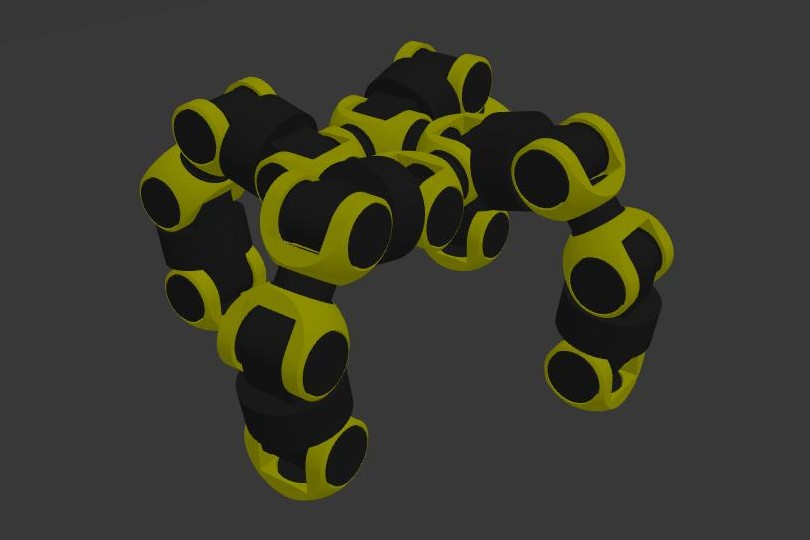
\includegraphics[width=.9\linewidth]{data/spider.jpg}
    \caption{RoFIbot in the spider configuration in the Gazebo simulation.}
    \label{fig:spider}
\end{figure}

The spider is the second iconic shape of the self-reconfigurable robots.
The wheel can move fast forward and backward, but the spider can move to any side at the same efficiency.
The spider's multiple legs offer the RoFIbot stable support when it is not moving, but the movement itself is much more complicated than in the wheel configuration.

Because of the complexity of the movement, there is no moving spider example.
Nevertheless, there is, a world \code{worlds/spider.in}, that shows the spider in its standing position.
The spider configuration can be seen in Figure \ref{fig:spider}.

\subsection{50 Modules}

The 50 modules world is showing the capabilities of the world creator tool.
The simulation of so many modules creates a high load on the server machine, so running the simulator in a paused state is recommended.

\subsection{Communication}

The communication example shows the RoFI networking inside the Gazebo simulation.
This example is currently the only example that requires a user program for each module in the simulation.
The example demonstrates the usage of packet sending between connected RoFI modules through RoFICoMs.


\section{Evaluation}

This thesis's work allows simulating the RoFI Universal Modules and provides an easy way to add new types of modules.
The simulation can mimic the behavior of the RoFICoM, its connective and disconnective properties, and it also simulates the packet transfer between two connected RoFI modules.

The RoFI Universal Module simulation seems reasonable, but at the time of writing, there is only one created physical RoFI Universal Module that is not even fully completed.
The simulation may need to be tweaked to represent the physical module accurately.

The simulation does not replicate the batteries and does not check for destructive forces on the RoFICoMs or other parts of the module.
It does, however, limit the force that the joints and RoFICoMs can produce.


\chapter{Conclusion}
% How I managed to make an awesome tool, that will help the world

This thesis is dealing with the RoFI simulator project.
The project's main goal is to create a tool to simulate the self-reconfigurable modular robots from the RoFI platform.
The simulator provides the same RoFI HAL interface as the physical modules and, at the same time, keeps the distributed nature of the RoFI platform.
Both of these factors make it easy to transition the code between the simulated and the physical modules.
It is especially important because the RoFI platform is in the early stages of the development and the simulation allows for a quick, cheap, and effective way of finding the right reconfiguring and movement algorithms.
So far, there are only a few simulators that deal with simulating self-reconfigurable robots and none of those are able to simulate the RoFI platform.

There are still improvements that can be added to the RoFI simulator to make it better.
The Protobuf messages in GazeboSim use the best-effort delivery and sometimes the command messages get lost.
This could be handled by some reliable protocol inside the Gazebo messaging system.
In regards to the capabilities of the RoFI Universal Module, the module provides a gravity sensor that could enable the balancing of a RoFIbot and a distance sensor inside each RoFICoM that could be used when scanning the environment.
Also, the controlling of the RoFI joints by velocity and position could be improved by tuning the PID constants' values.

There is still plenty of work ahead before the simulation of the RoFI platform adequately represents the physical RoFI modules.
Nevertheless, the RoFI simulator has a lot of potential in helping with the growth of the RoFI platform.
Even at the time of writing this thesis, the simulator is already being used in the development of RoFI networking.

The implementation part of this thesis is a part of the RoFI GitHub repository available at https://github.com/paradise-fi/RoFI .
A copy of the repository is available as the attachment.
The project of this thesis is fully contained in the directory \code{RoFI/simulator}.
Only the subdirectory \code{hal/lwip} and the example \code{communication} are related to networking and were created by another member of the RoFI team.

\end{document}
